%--------------------
% Packages
% -------------------
\documentclass[12pt,a4paper,titlepage]{article}
\usepackage[toc,page]{appendix}
\usepackage{amssymb, amsmath}
\usepackage[pdftex]{graphicx}
\usepackage[pdftex,linkcolor=black,pdfborder={0 0 0}]{hyperref}
\usepackage{calc}
\usepackage{tikz}
\usetikzlibrary{shapes.geometric, arrows}
\tikzstyle{startstop} = [rectangle, rounded corners, minimum width=3cm, minimum height=1cm,text centered, draw=black, fill=red!30]
\tikzstyle{io} = [trapezium, trapezium left angle=70, trapezium right angle=110, minimum width=3cm, minimum height=1cm, text centered, draw=black, fill=blue!30]
\tikzstyle{process} = [rectangle, minimum width=3cm, minimum height=1cm, text centered, draw=black, fill=orange!30]
\tikzstyle{decision} = [diamond, minimum width=3cm, minimum height=1cm, text centered, draw=black, fill=green!30]
\tikzstyle{arrow} = [thick,->,>=stealth]

\usepackage{enumitem}
\linespread{1.2} % Set linespace
\usepackage[a4paper, lmargin=0.1666\paperwidth, rmargin=0.1666\paperwidth, tmargin=0.1111\paperheight, bmargin=0.1111\paperheight]{geometry} %margins
\usepackage{graphicx}
\usepackage{nomencl}
\makenomenclature

\title{\Huge \underline{ Decision Theory and Design Optimisation}}
\author{Debjit Hore.}
\date{\today}
%-----------------------
% Begin document
%-----------------------
\begin{document}
\maketitle
\mbox{}
\nomenclature{\(E\)}{Young's modulus (MPa)}
\nomenclature{\(A\)}{Area of cross-section (m$^{2}$)}
\nomenclature{\(\boldsymbol{\sigma}\)}{Stress tensor}
\printnomenclature

\clearpage
\tableofcontents

\clearpage
\section{\underline{Introduction}}
``Mathematics is the language with which God wrote the universe"-Galileo.\\[1\baselineskip]
Optimisation is the process of maximising or minimising a desired objective function, while satisfying the prevailing constraints. Nature has infinite examples where an optimum state of the system is sought. As such the application of ``optimisation'' can be seen in nature as well as human creations. Some common examples are as follows:
{\begin{enumerate}
    \item A liquid droplet in zero gravity attaining a perfect sphere shape to minimise surface area for a given volume.
    \item Naturally occurring honeycomb structures ( which humans have effectively implemented and used ) are one of the most compact packaging arrangements.\
    \item Genetic mutation for survival is another natural optimisation process.
    \item Modern Machine Learning techniques are geared towards minimising a given `cost function' thereby minimising error.
\end{enumerate}}

\subsection{\underline{Brief history of Optimisation.}}
\begin{enumerate}
    \item Euclid of Alexandria (325-265 BCE) solved early optimisation problems in geometry.
    \item Heron of Alexandria (10-75 CE) showed that light travels between points through the path of shortest length.
    \item Pappus of Alexandria (290–350 CE), among his many contributions to optimization, argued that the hexagon repeated in honeycomb is the optimal regular polygon for storing honey; its hexagonal structure uses the least material to create a lattice of cells over a plane.
    \item The use of a gradient method (requiring derivatives of the functions) for minimization was first presented by Cauchy in 1847. 
    \item Karush, Kuhn, and Tucker who derived the “KKT” optimality conditions for constrained problems [1939, 1951]. Thereafter,particularly in the 1960s, several numerical methods to solve nonlinear optimization problems were developed.
    \item Methods for unconstrained minimization include conjugate gradient methods of Fletcher and Reeves [1964] and the variable metric methods of Davidon–Fletcher–Powell (DFP) in [1959].
    \item  Rosenbrock's method of orthogonal directions [1960], simplex method of Nelder and Meade [1965]. 
    \end{enumerate}
    
%
\subsection{\underline{Flow of an Optimisation Problem.}}
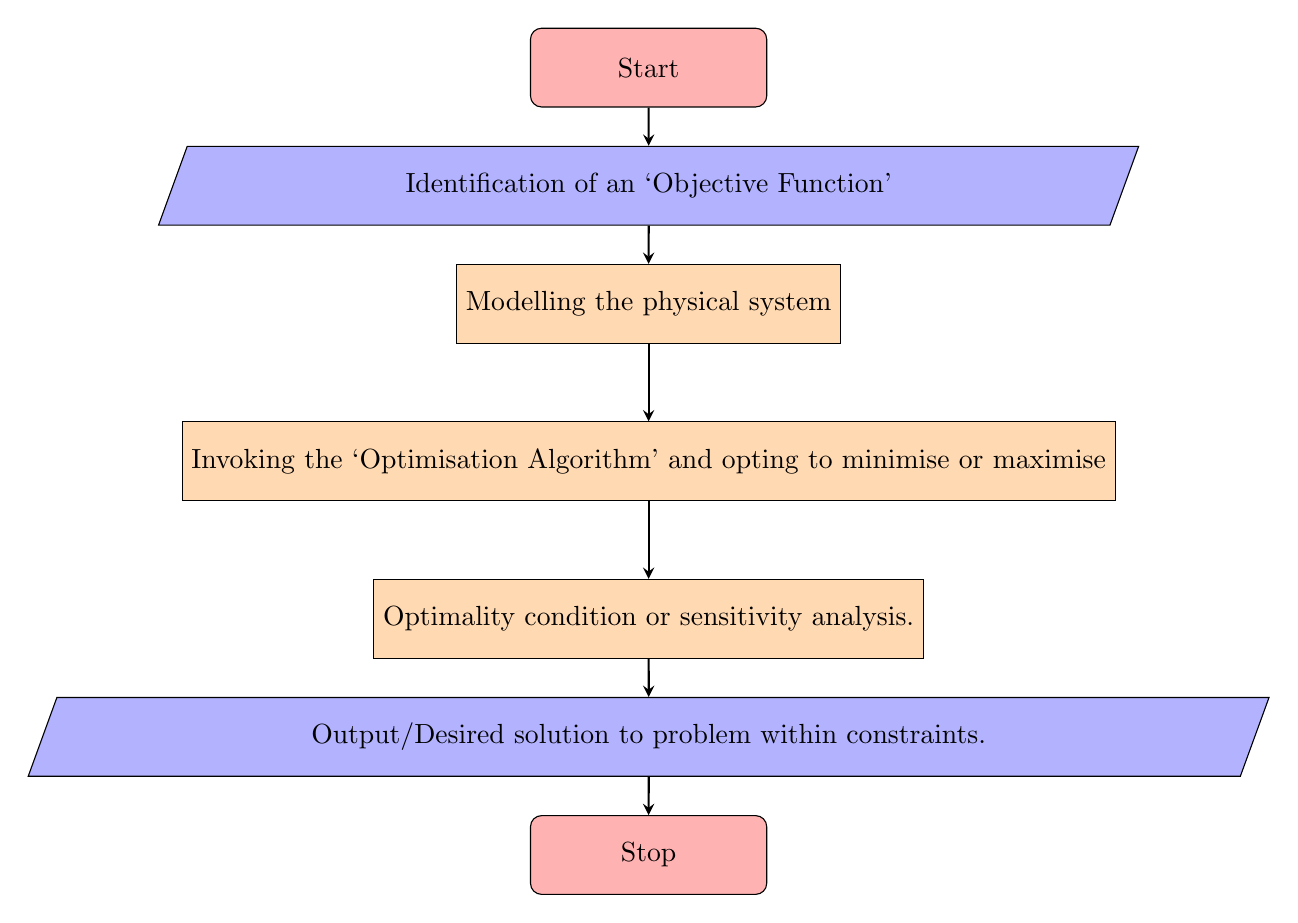
\begin{tikzpicture}[node distance=1.5 cm]
\node (start) [startstop] {Start};
\node (in1) [io, below of=start] {Identification of an `Objective Function'};
\node (pro1) [process, below of=in1] {Modelling the physical system};
\node (pro2) [process, below of=pro1, yshift=-0.5cm] {Invoking the `Optimisation Algorithm' and opting to minimise or maximise};
\node (pro3) [process, below of=pro2, yshift=-0.5cm] {Optimality condition or sensitivity analysis.};
\node (out1) [io, below of=pro3] {Output/Desired solution to problem within constraints.};
\node (stop) [startstop, below of=out1] {Stop};
\draw [arrow] (start) -- (in1);
\draw [arrow] (in1) -- (pro1);
\draw [arrow] (pro1) -- (pro2);
\draw [arrow] (pro2) -- (pro3);
\draw [arrow] (pro3) -- (out1);
\draw [arrow] (out1) -- (stop);
\end{tikzpicture}

You should add the citations as described here \cite{sadd2009elasticity}. You can refer to this document for more latex symbols\footnote{https://wch.github.io/latexsheet/}.
%

\subsection{\underline{Types of Problems:}}
\begin{enumerate}
    \item Linear Programming.
    \item Integer Programming.
    \item 0-1 Programming.
    \item Mixed Integer Programming. (MIP)
    \item Mixed Integer Non-Linear Programming. (MINLP)
    \item Quadratic Programming.
    \item Convex Programming. (Local solution is Global solution)
    \item Combinatorial Problems.
\end{enumerate}
%

\section{Unconstrained Optimisation}

\subsection{\underline{First Order Necessary Condition.}}
For unconstrained optimisation, if x* is a local minimiser, then the rate of increase of function \textbf{f} at x* in any feasible direction \textbf{\underline{d}} in the feasible region $\Omega$ is non-negative :

\begin{equation}
    \dfrac{\partial f}{\partial\underline{d} } \geq 0 \label{eq1} 
\end{equation}
For an interior point of $\Omega$ if x* is local minimiser then :
\begin{equation}
    \nabla f (x*)=  0 \label{eq2} 
\end{equation}


\subsection{\underline{Second Order Necessary Condition.}}
For \textbf{SONC}, x* is a local minimiser of \textbf{f} over $\Omega$ and \textbf{\underline{d}} is a feasible direction if:

\begin{equation}
    \underline{d}^T \nabla f(x*)= 0 \label{eq3}
\end{equation}
\textbf{then}
\begin{equation}
    \underline{d}^T \textbf{H(x*)} \underline{d} \geq 0 \label{eq4}
\end{equation}
where H(x*) is the Hessian of f at x*.

\subsection{\underline{Second Order Sufficient Condition}}
Suppose \textbf{\underline{f}} is a function from \textbf{R^n $\rightarrow$ R} is twice differentiable such that 
\begin{equation}
    \nabla f(x*)=0    
\end{equation}
and
\begin{equation}
    \textbf{H(x*)} > 0
\end{equation}
then x* is a strict local minimiser of \textbf{f}.

\subsection{\underline{One Dimensional Unconstrained Optimisation.}}
1D problem is defined as:
minimise\textbf{(f), f:R$\rightarrow$R} when $\Omega$ = \textbf{R}, where $\Omega$ is the domain of \textbf{f}.
The approach is to use an iterative search algorithm also called a `line-search' method. \\
\textbf{Linear Search Algorithms}: 
\begin{enumerate}
    \item Golden Section Method.
    \item Fibonacci Method.
    \item Bisection Method.
    \item Secant Method.
    \item Newton's Method
\end{enumerate}

A sample image (Fig. \ref{fig1}) shows how a typical line search algorithm works: 
\begin{figure}[h!tb]
	\centering
	\includegraphics[scale=1]{line_searchdemo.png}
	\caption{Typical Linear Search Algorithm} \label{fig1}
\end{figure}
\\
\textbf{\underline{Unimodality}} of the objective function is an important assumption in most of these line-search algorithms, which means there is an unique x* such that \emph{f} is monotonically decreasing for x $\leq$ x* and monotonically increasing for x $\geq$ x*, which means there is a \textbf{unique} global minimum.
\subsubsection{\underline{Golden Section Method}}
Target: To find argmin(\textbf{f}) over a closed interval $[a^0, b^0]$ where \textbf{f :R$\rightarrow$R} and a unimodal function.
\begin{enumerate}
    \item Choose $[a^1, b^1]$ such that $a^1-a^0=b^0-b^1=\rho(b^0-a^0)$
    \item If $f(a^1) < f(b^1)$ then minimiser in range $[a^0, b^1]$ else in range $[a^1,b^0]$
    \item Start with reduced range of uncertainty and repeat the process.
\end{enumerate}
Here $\rho$ is the golden ratio and equals 0.61803
\subsubsection{\underline{Fibonacci Method}}
In Fibonacci, we vary the value of $\rho$ at every step, such that the updation rule is as follows:
\begin{equation}
   \rho_{k+1}= 1- \rho_{k}/(1-\rho_{k})
\end{equation}
\subsubsection{\underline{Bisection Method}}
\begin{enumerate}
    \item For starters, $x^0$ is chosen such that $x^0=(a^0+b^0)/2$
    \item Evaluate $f'(x^0)$.
    \item If this value is less than 0 then x* (minimiser) lies right of $x^0$ and interval is reduced to $[x^0, b^0]$, or else $[a^0, x^0]$ 
    \item If $f'(x^0)$ =0, then x*= $x^0$, search is terminated.
\end{enumerate}
\subsection{Subsection}
You can refer to Eq. \ref{eq2} in the text as described here.
%
\begin{equation}
    EA \dfrac{\partial^{2} u}{\partial x^{2}} = 0 \label{eq2}
\end{equation}
%
%
\begin{equation}
    \nabla \cdot \boldsymbol{\sigma} + \boldsymbol{f} = \mathbf{0} \label{eq3}
\end{equation}
%
The equation (\ref{eq3}) can also be written as:
%
\begin{equation}
    \mathrm{Div} \ \boldsymbol{\sigma} + \boldsymbol{f} = \mathbf{0} \label{eq4}
\end{equation}
%
%
\clearpage
\bibliographystyle{unsrt}
\bibliography{sample}
\end{document}